\documentclass{beamer}
\usepackage{latexsym}
\usepackage{graphicx}
\usetheme{Warsaw}

\title{Chapter 5}
\subtitle{Dimensionality Reduction}

\begin{document}
\maketitle

\begin{frame}
  \frametitle{Principal Component Analysis (PCA)}
  \begin{columns}[c]
    \column{0.5\textwidth}
    \begin{itemize}
    \item Find the directions of maximum variance
    \item Project data onto the lower-dimensional space
    \item Original features: $x_1$ and $x_2$
    \item Principal components: \textbf{PC1} and \textbf{PC2}
    \end{itemize}
    \column{0.5\textwidth}
    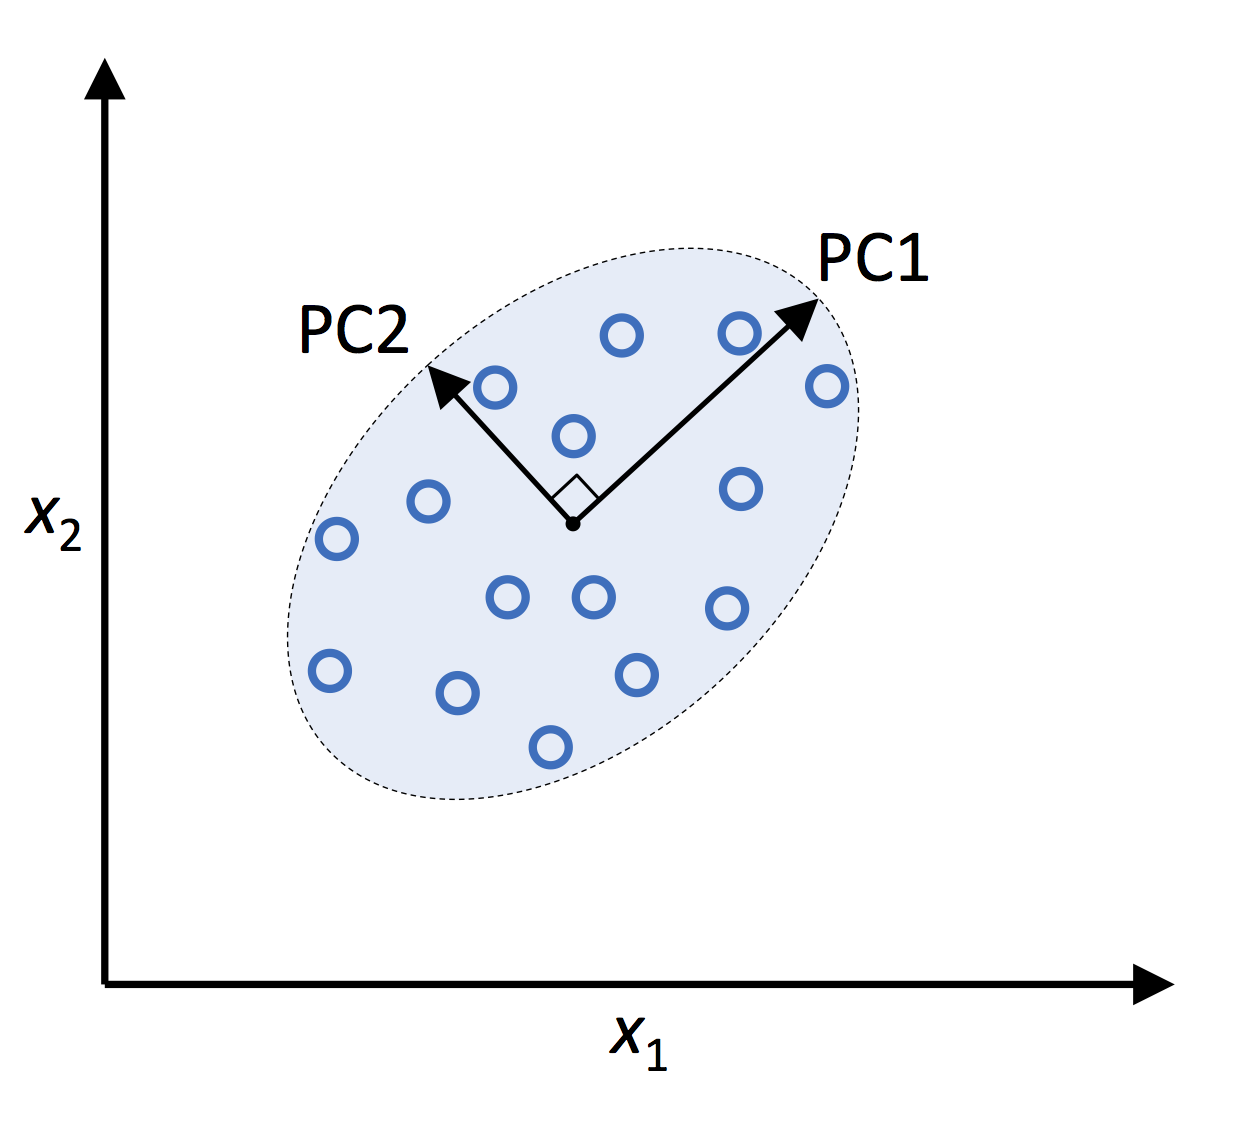
\includegraphics[width=\textwidth]{Code/ch05/images/05_01.png}
  \end{columns}
\end{frame}

\begin{frame}
  \frametitle{Mapping to a low-dimensional space}
  When we use PCA for dimensionality reduction, we construct a $d \times k$ transformation matrix $\mathbf{W}$.
  We then map a sample vector $\mathbf{x}$ onto a new $k$-dimensional feature subspace ($k << d$)
  \[
  \mathbf{x} = [ x_1, x_2, \dots, x_j], \mathbf{x} \in \mathbb{R}^d
  \]
  \[
  \downarrow \mathbf{x W}, \quad \mathbf{W} \in \mathbb{R}^{d \times k}
  \]
  \[
  \mathbf{z} = [z_1, z_2, \dots, z_k], \quad \mathbf{z} \in \mathbb{R}^k
  \]
\end{frame}

\begin{frame}
  \frametitle{Principal components}
  \begin{itemize}
  \item Transforming $d$-dimensional data to $k$ dimensions
  \item First principal component will have the largest variance
  \item Second principal component will have next largest variance
  \item And so on...
  \item PCA sensitive to data scaling, so need to standardize features
  \end{itemize}
\end{frame}

\begin{frame}
  \frametitle{Algorithm}
  \begin{enumerate}
  \item Standardize the $d$-dimensional dataset.
  \item Construct the covariance matrix.
  \item Decompose the covariance matrix into its eigenvectors and eigenvalues.
  \item Select $k$ eigenvectors that correspond to the $k$ largest eigenvalues, where $k$ is the dimensionality of the new feature subspace $(k \le d)$.
  \item Construct a projection matrix $\mathbf{W}$ from the "top" $k$ eigenvectors.
  \item Transform the $d$-dimensional input dataset $\mathbf{X}$ using the projection matrix $\mathbf{W}$ to obtain the new $k$-dimensional feature subspace.
  \end{enumerate}
\end{frame}

\begin{frame}
  \frametitle{Variance-covariance matrix}
  \begin{itemize}
  \item Symmetric $d \times d$ -dimensional matrix ($d$ - number of dimensions)
  \item Pairwise covariances between the different features
  \item Covariance between two features $\mathbf{x}_j$ and $\mathbf{x}_k$:
    \[
    \sigma_{jk} = \frac{1}{n} \sum_{i=1}^{n} \big(  x_{j}^{(i)} - \mu_j  \big) \big(  x_{k}^{(i)}  - \mu_k \big)
    \]
    Where $\mu_j$ and $\mu_k$ are the sample means of feature $j$ and $k$
  \end{itemize}

\end{frame}

\begin{frame}
  \frametitle{What is covariance?}
  \begin{itemize}
  \item Measure of how much two random variables change together
  \item Positive covariance
    \begin{itemize}
    \item Features increase together
    \item Features decrease together
    \item E.g. As a balloon is blown up it gets larger in all dimensions
    \end{itemize}
  \item Negative covariance
    \begin{itemize}
    \item Features vary in opposite directions
    \item Large values of one variable correspond to small values of the other
    \item E.g. if a sealed balloon is squashed in one dimension then it will expand in the other two
    \end{itemize}
  \item The magnitude of the covariance is not easy to interpret
  \item The normalized version of covariance (\textit{correlation coefficient})  indicates the strength of the linear relation.
  \end{itemize}
\end{frame}

\begin{frame}
  \frametitle{Variance-covariance matrix}
  \begin{itemize}
  \item For three features, covariance matrix will look like this:
    \[
    \Sigma = \begin{bmatrix}
      \sigma_{1}^2 & \sigma_{12} & \sigma_{13} \\
      \sigma_{21} & \sigma_{2}^{2} & \sigma_{23} \\
      \sigma_{31} & \sigma_{32} & \sigma_{3}^{2}
    \end{bmatrix}
    \]
  \item The eigenvectors of $\Sigma$ represent the principle components
  \item The corresponding eigenvalues represent their magnitude
    \begin{itemize}
    \item Principle components: the directions of maximum variance
    \end{itemize}
  \item E.g. Wine dataset (13 dimensions)
    \begin{itemize}
    \item $13x13$ covariance matrix
    \item 13 eigenvectors
    \item 13 eigenvalues
    \end{itemize}
  \end{itemize}
\end{frame}

\begin{frame}
  \frametitle{Eigenpairs}
  \begin{itemize}
  \item An Eigenvector $\mathbf{v}$ satisfies the condition:
    \[
    \Sigma \mathbf{v} = \lambda \mathbf{v}
    \]
    Where $\lambda$ is the eigenvalue (scalar)
  \item NumPy has a function to compute eigenpairs
  \item We want to reduce the dimensionality
  \item So, we select a subset of $k$ most informative eigenvectors
  \end{itemize}
\end{frame}

\begin{frame}
  \frametitle{Variance explained ratio}
  \begin{itemize}
  \item Variance explained ratio of an eigenvalue $\lambda_j$:
  \[
  \frac{\lambda_j}{\sum_{j=1}^{d} \lambda_j}
  \]
  \item First two principal components explain about 60 percent of the variance in the data
  \end{itemize}
  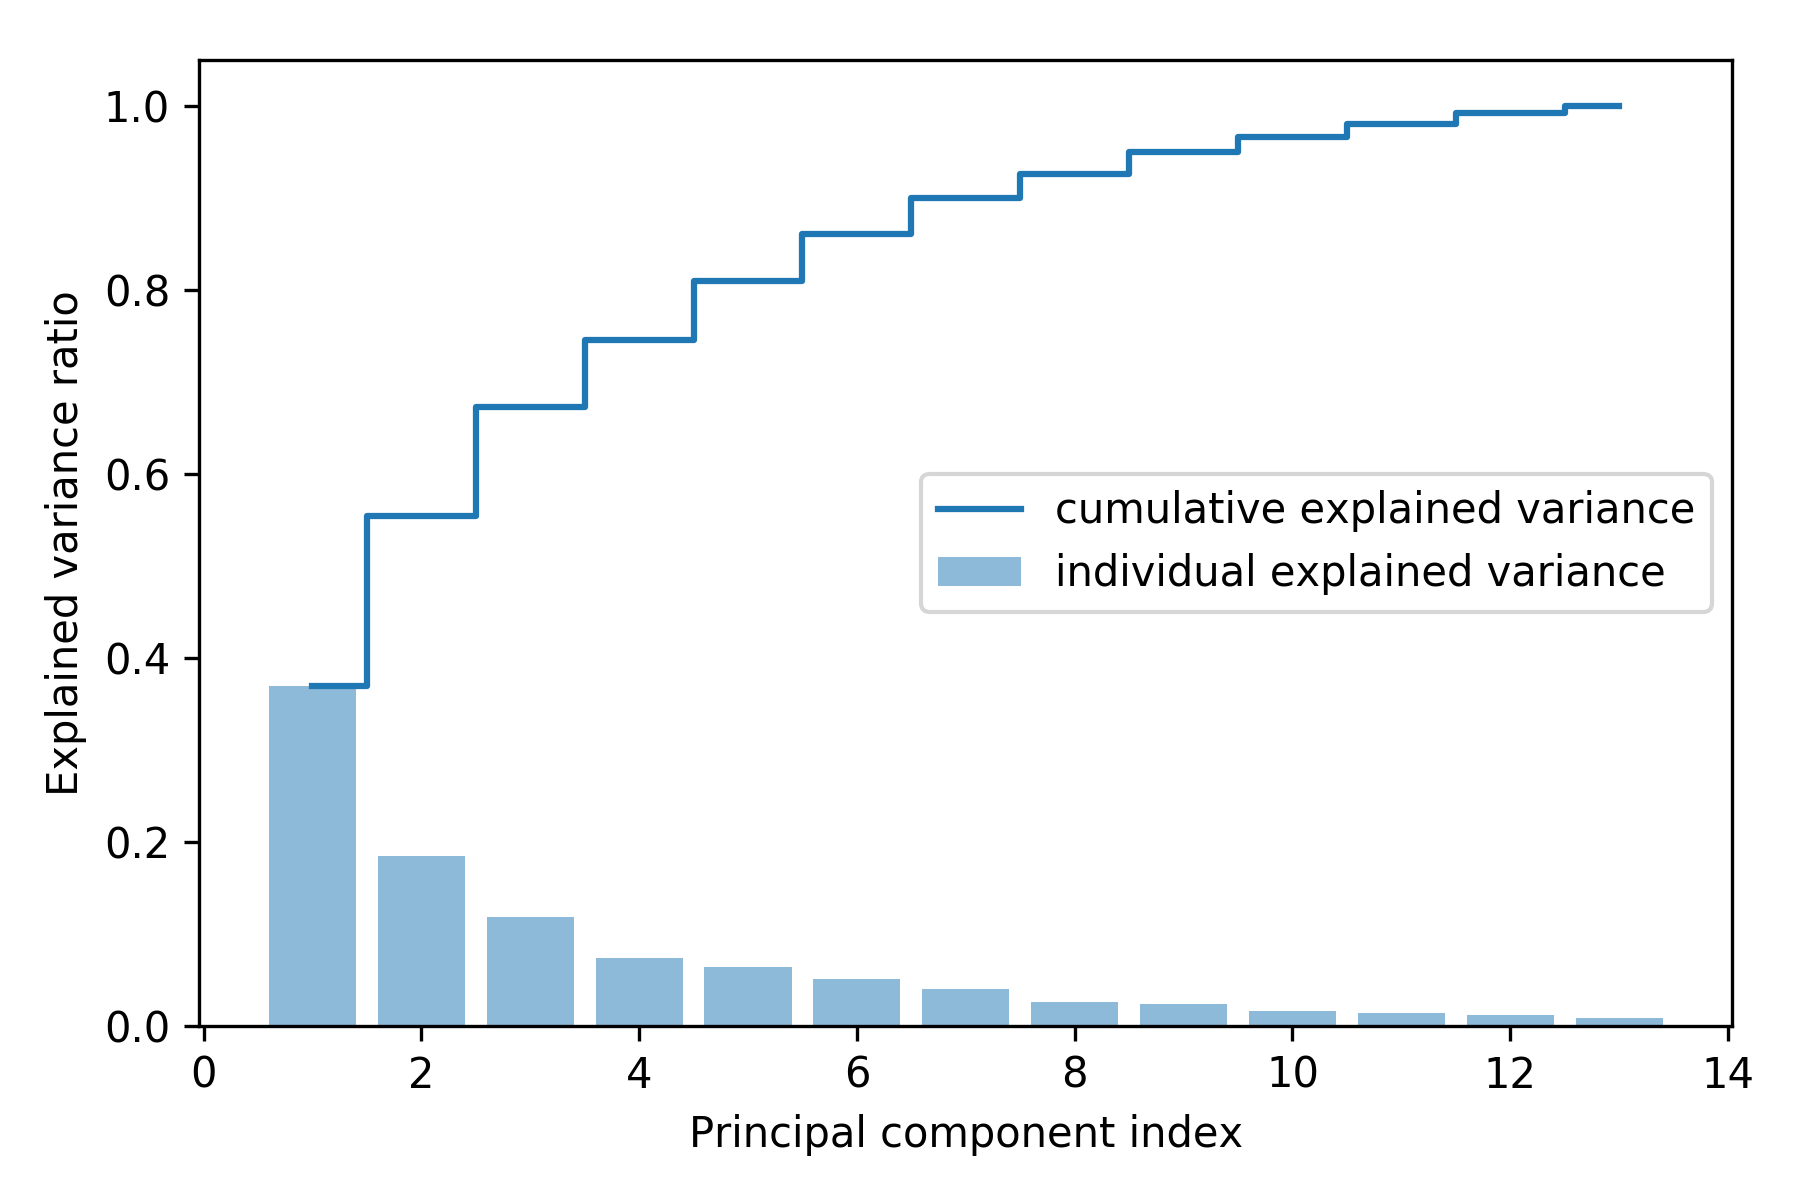
\includegraphics[scale=0.55]{Code/ch05/images/05_02.png}
\end{frame}

\begin{frame}
  \frametitle{Feature transformation}
  \begin{itemize}
  \item We decomposed the covariance matrix into eigenpairs
  \item Now need to project to new space defined by principle component axes
  \item Construct a $13 \times 2$ projection matrix from top two eigenvectors
  \item Transform a sample $\mathbf{x}$ onto the PCA subspace obtaining $\mathbf{x}'$
  \item Which is a two-dimensional vector consisting of two new features:
    \[
    \mathbf{x}' = \mathbf{xW}
    \]
  \item Transform entire Wine dataset ($124 \times 13$)
    \[
    \mathbf{X}' = \mathbf{XW}
    \]
  \end{itemize}
\end{frame}

\begin{frame}
  \frametitle{Visualize \textit{Wine} dataset in two dimensions}
  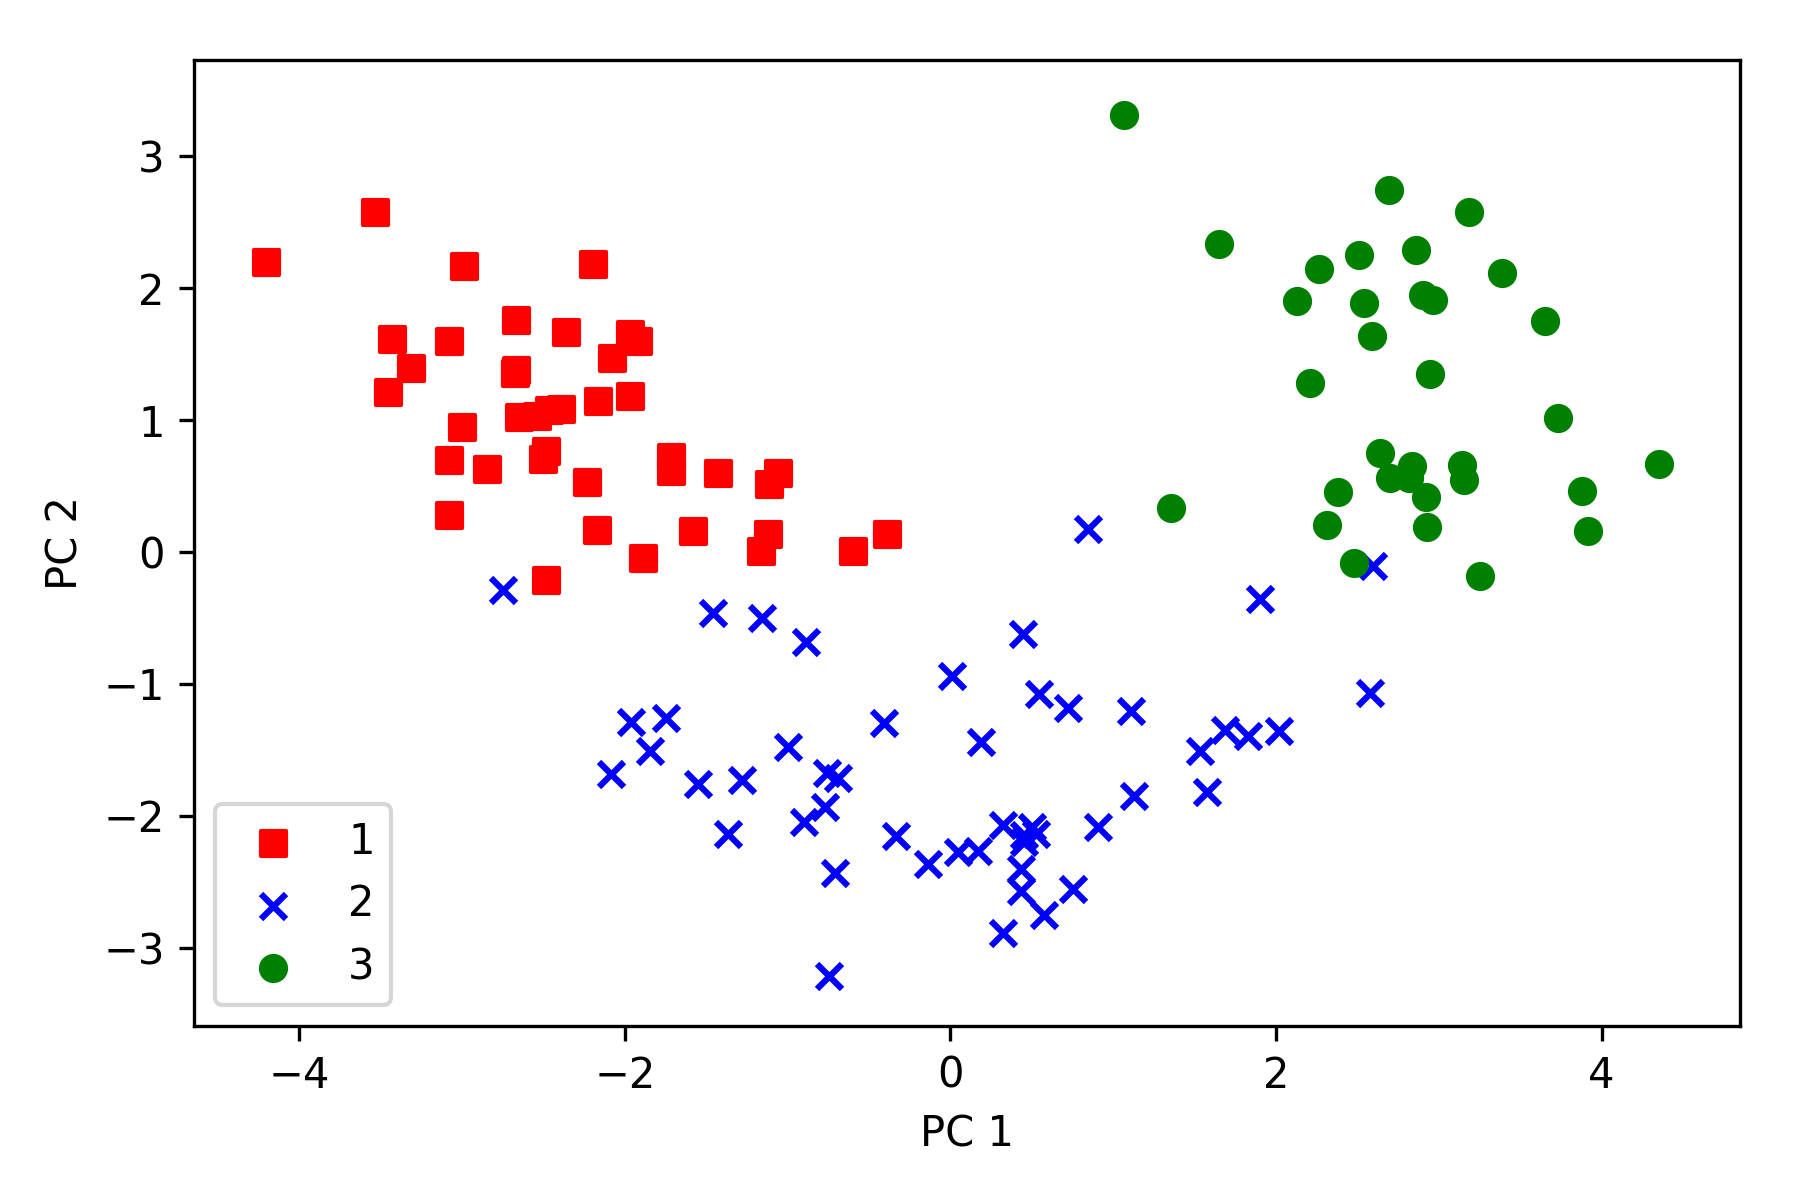
\includegraphics[scale=0.55]{Code/ch05/images/05_03.png}
\end{frame}

\begin{frame}
  \frametitle{Visualize \textit{Wine} dataset in two dimensions}
  \begin{columns}[c]
    \column{0.5\textwidth}
    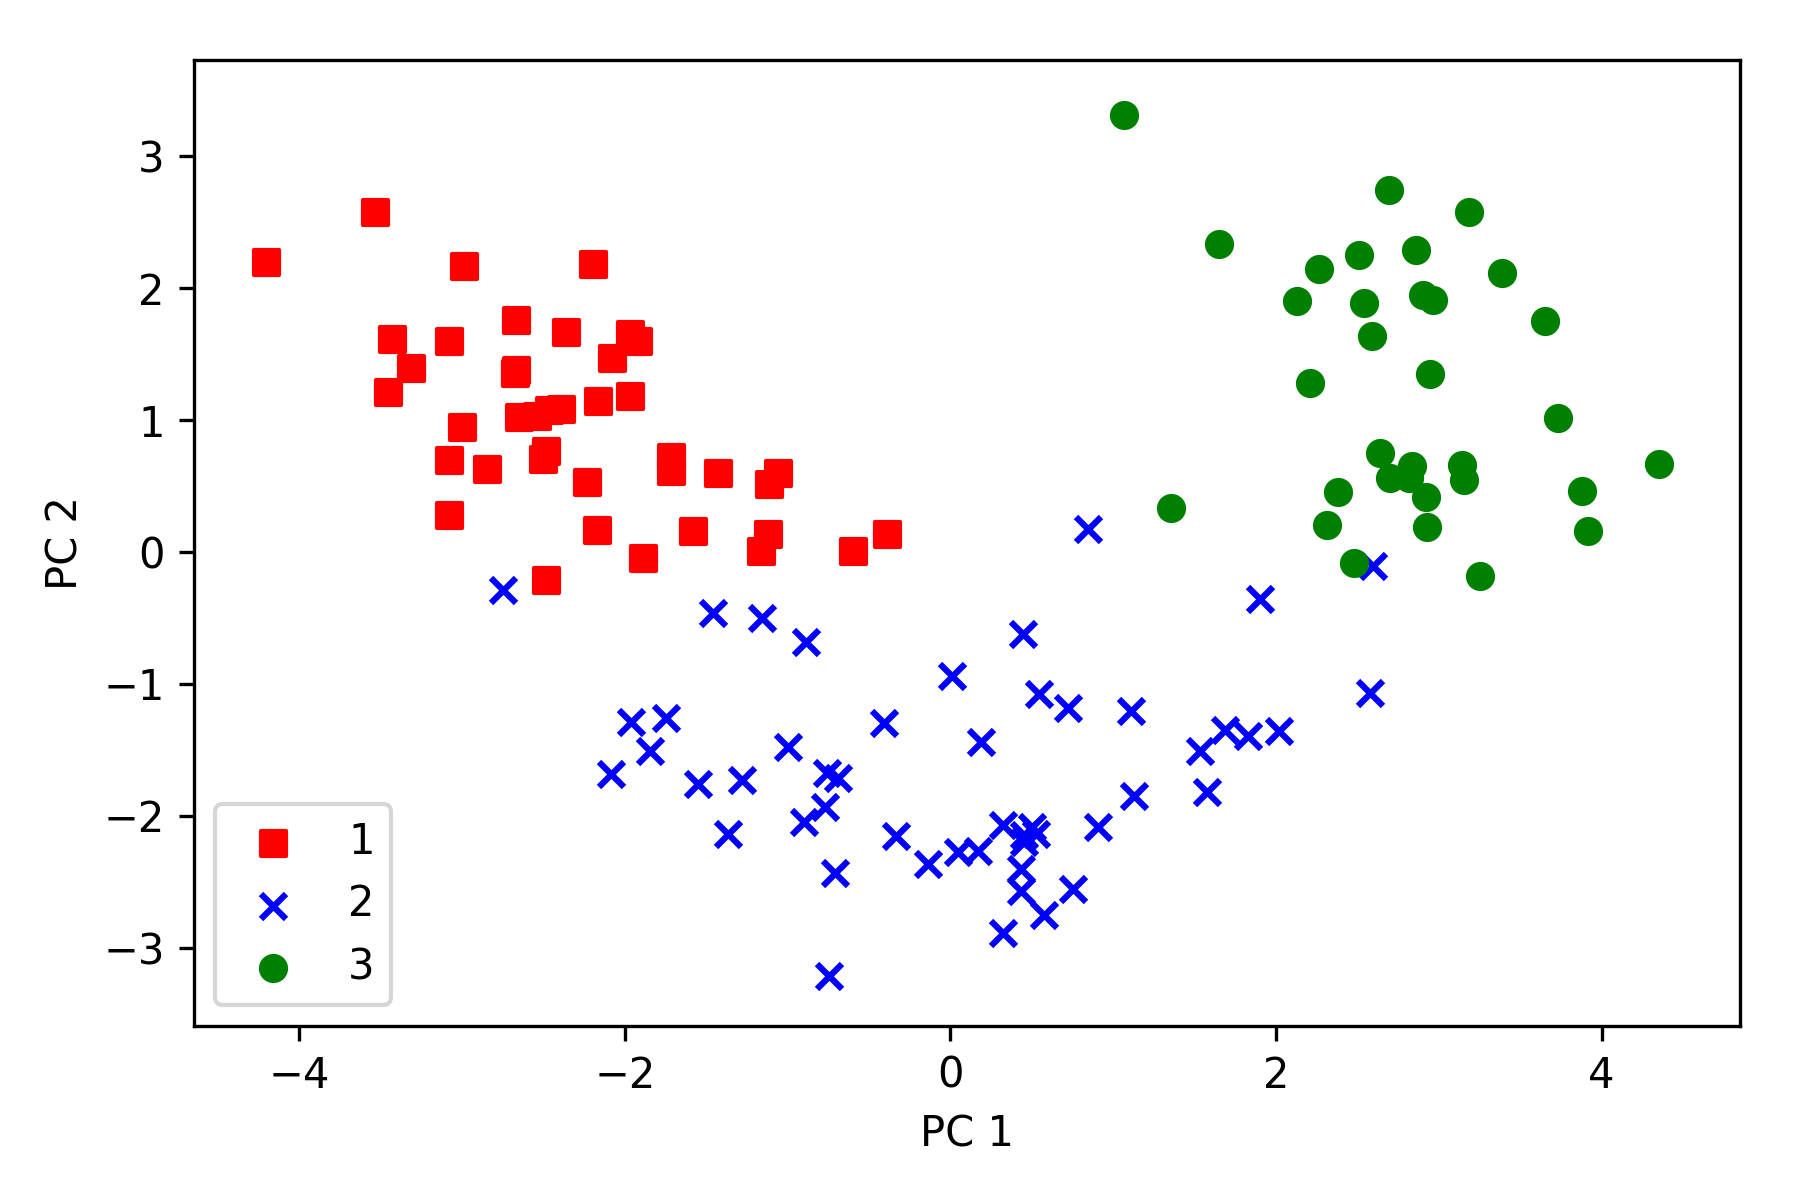
\includegraphics[scale=0.35]{Code/ch05/images/05_03.png}
    \column{0.5\textwidth}
    \begin{itemize}
    \item Can now visualize a 13-dimensional dataset
    \item Data more spread along first principal component, which explained 40 percent of the variance
    \item A linear classifier should be able to do a good job separating the classes
    \item Keep in mind that PCA is an \textit{unsupervised} algorithm
    \end{itemize}
  \end{columns}
\end{frame}

\end{document}
